%
% frame.tex
%
% (c) 2019 Prof Dr Andreas Müller, Hochschule Rapperswil
%

%
% Definition Frame
%
\begin{frame}
\frametitle{Frame}
\begin{definition}
Eine Menge von Vektoren $a_j$ heisst {\em Frame}, wenn
es Zahlen $B\ge A>0$ gibt mit
\[
A \|x\|^2
\le
\sum_{j} |\langle x,a_j\rangle|^2
\le
B \|x\|^2
\]
\uncover<2->{%
Das Frame heisst {\em straff}, wenn $A=B$.
}
\end{definition}
\begin{columns}[T,totalwidth=\textwidth]
\begin{column}{0.48\linewidth}
\uncover<3->{%
\begin{block}{Orthonormalbasis}
Falls $\mathcal{B}$ eine orthonormierte Basis,
dann ist $\mathcal{B}$ ein straffes Frame mit
$A=B=1$.
\end{block}
}
\end{column}
\uncover<4->{%
\begin{column}{0.48\linewidth}
\begin{block}{Mehrere Orthonormalbasen}
Falls $\mathcal{B}_i$ ein o.n.~Basis ist $1\le i\le n$,
dann ist
\[
\mathcal{B}
=
\bigcup_i \mathcal{B}_i
\]
ein straffes Frame mit $A=B=n$.
\end{block}
}
\end{column}
\end{columns}

\end{frame}

%
%
%
\begin{frame}
\frametitle{Dreiecksframe}
\centering
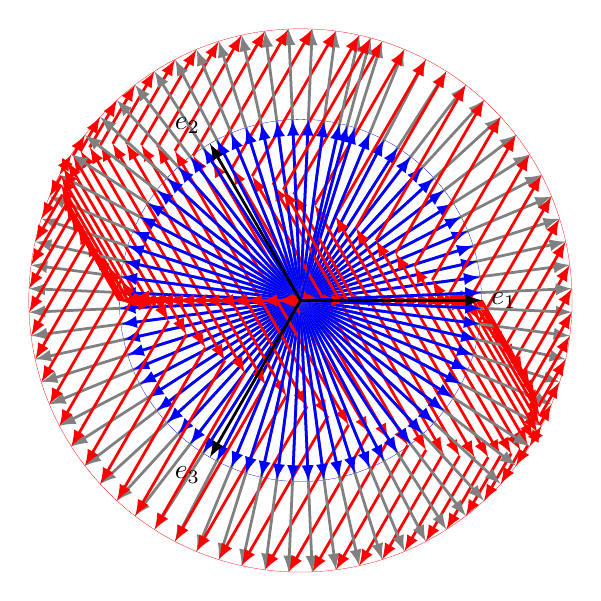
\begin{tikzpicture}[>=latex,scale=2.3]

\draw[color=red,line width=0.1pt] (0,0) circle[radius=1.5];
\draw[color=blue,line width=0.1pt] (0,0) circle[radius=1.0];

\ifthenelse{\boolean{presentation}}{
\foreach \A in {1,...,72}{
	\pgfmathparse{2.5+\A*5}
	\xdef\a{\pgfmathresult}

	\only<\A>{
	\draw[->,color=gray,line width=1pt] (0,0)--({1.5*cos(\a)},{1.5*sin(\a)});
	\draw[->,color=blue,line width=1pt] (0,0)--({cos(\a)},{sin(\a)});
	\pgfmathparse{cos(\a)}
	\xdef\x{\pgfmathresult}
	\pgfmathparse{sin(\a)}
	\xdef\y{\pgfmathresult}
	\draw[->,color=red,line width=1pt]
		(0,0)--({\x},0);
	\pgfmathparse{(-0.5)*\x+\y*(sqrt(3)/2)}
	\xdef\B{\pgfmathresult}
	\pgfmathparse{(-0.5)*\x+\y*(-sqrt(3)/2)}
	\xdef\C{\pgfmathresult}
	\draw[->,color=red,line width=1pt]
		({\x},0)--({\x-0.5*\B},{0+\B*sqrt(3)/2});
	\draw[->,color=red,line width=1pt]
		({\x-0.5*\B},{0+\B*sqrt(3)/2})
		--({\x-0.5*\B-0.5*\C},{0+\B*sqrt(3)/2-\C*sqrt(3)/2});
	}
}
}{
	\xdef\a{75}

	\draw[->,color=gray,line width=1pt] (0,0)--({1.5*cos(\a)},{1.5*sin(\a)});
	\draw[->,color=blue,line width=1pt] (0,0)--({cos(\a)},{sin(\a)});
	\pgfmathparse{cos(\a)}
	\xdef\x{\pgfmathresult}
	\pgfmathparse{sin(\a)}
	\xdef\y{\pgfmathresult}
	\draw[->,color=red,line width=1pt]
		(0,0)--({\x},0);
	\pgfmathparse{(-0.5)*\x+\y*(sqrt(3)/2)}
	\xdef\B{\pgfmathresult}
	\pgfmathparse{(-0.5)*\x+\y*(-sqrt(3)/2)}
	\xdef\C{\pgfmathresult}
	\draw[->,color=red,line width=1pt]
		({\x},0)--({\x-0.5*\B},{0+\B*sqrt(3)/2});
	\draw[->,color=red,line width=1pt]
		({\x-0.5*\B},{0+\B*sqrt(3)/2})
		--({\x-0.5*\B-0.5*\C},{0+\B*sqrt(3)/2-\C*sqrt(3)/2});
}

\draw[->,line width=1pt] (0,0)--(1,0);
\draw[->,line width=1pt] (0,0)--(-0.5,{sqrt(3)/2});
\draw[->,line width=1pt] (0,0)--(-0.5,{-sqrt(3)/2});
\node at (1,0) [right] {$e_1$};
\node at (-0.5,{sqrt(3)/2}) [above left] {$e_2$};
\node at (-0.5,{-sqrt(3)/2}) [below left] {$e_3$};
\end{tikzpicture}
\end{frame}

%
%
%
\begin{frame}
\frametitle{Straffe Frames}
Gram-Operator:
\[
Gx = \sum_{j} \langle x,a_j\rangle a_j
\]
\end{frame}
